%%% LaTeX Template
%%% This template is made for project reports
%%%	You may adjust it to your own needs/purposes
%%%
%%% Copyright: http://www.howtotex.com/
%%% Date: March 2011

%%% Preamble
\documentclass[paper=a4, fontsize=12pt]{scrartcl}	% Article class of KOMA-script with 12pt font and a4 format


\usepackage[english]{babel}				% English language/hyphenation
\usepackage[protrusion=true,expansion=true]{microtype}	% Better typography
\usepackage{amsmath,amsfonts,amsthm}			% Math packages
\usepackage[pdftex]{graphicx}				% Enable pdflatex
\usepackage{url}
\usepackage[margin=1.5in]{geometry}
\usepackage{algorithm}
\usepackage{algorithmic}
\usepackage{framed}
\usepackage{listings}
\usepackage{color}
\usepackage{textcomp}

\definecolor{listinggray}{gray}{0.9}
\definecolor{lbcolor}{rgb}{0.98,0.98,0.98}
\lstset{
backgroundcolor=\color{lbcolor},
tabsize=4,
rulecolor=,
language=matlab,
basicstyle=\footnotesize\ttfamily,
upquote=true,
aboveskip={1.5\baselineskip},
columns=fixed,
showstringspaces=false,
extendedchars=true,
breaklines=true,
prebreak = \raisebox{0ex}[0ex][0ex]{\ensuremath{\hookleftarrow}},
frame=single,
showtabs=false,
showspaces=false,
showstringspaces=false,
identifierstyle=\ttfamily,
keywordstyle=\color[rgb]{0,0,1},
commentstyle=\color[rgb]{0.133,0.545,0.133},
stringstyle=\color[rgb]{0.627,0.126,0.941},
numbers=left
}


%%% Custom sectioning (sectsty package)
\usepackage{sectsty}					% Custom sectioning (see below)
\allsectionsfont{\normalfont\scshape}			% Change font of al section commands


%%% Custom headers/footers (fancyhdr package)
\usepackage{fancyhdr}
\pagestyle{fancyplain}
\fancyhead{}						% No page header
%\fancyfoot[L]{\small \url{HowToTeX.com}}		% You may remove/edit this line 
\fancyfoot[C]{}						% Empty
\fancyfoot[R]{\thepage}					% Pagenumbering
\renewcommand{\headrulewidth}{0pt}			% Remove header underlines
\renewcommand{\footrulewidth}{0pt}			% Remove footer underlines
\setlength{\headheight}{13.6pt}


%%% Equation and float numbering
\numberwithin{equation}{section}		% Equationnumbering: section.eq#
\numberwithin{figure}{section}			% Figurenumbering: section.fig#
\numberwithin{table}{section}				% Tablenumbering: section.tab#


%%% Maketitle metadata (Defines how everything above the body should look like: title, header, authors, date, etc..)
\newcommand{\horrule}[1]{\rule{\linewidth}{#1}} 	% Horizontal rule

\title{
\vspace{-1in} 	
\usefont{OT1}{bch}{b}{n}
\normalfont \normalsize \textsc{University of Edinburgh - School of Informatics}
\\ [25pt]
\horrule{0.5pt} \\[0.4cm]
\large IAR - Task 3 Report \\
\horrule{1pt} \\[0.5cm]
}
\author{
  \normalfont \normalsize
  Jakob Calero - s0948339\\[-3pt]\normalsize
  Samuel Neugber - s0821562\\[-3pt]\normalsize
  \today
}
\date{}


%%% Begin document
\begin{document}
\maketitle					% Insert the title here
\section{Abstract}
Even with the limited information which can be extracted from the Khepera II robot's IR-sensors, particle filters can successfully estimate the location and orientation of said robot in a static arena. Using potential field navigation and stochastic exploration in the arena, in combination with the localisation from the particle filter, we were able to reliably find marked positions, return to the starting position and repeat this process several times in a few minutes. The system does have a few drawbacks, largely dominated by speed of execution, with some navigation fallacies as well as unreliability of finding marked positions due to stochastic exploration, but overall the methods we implemented work well together and get the job done as specified.

\section{Introduction}
In this final assignment we are given the task to put together our experience in navigation and control from previous tasks and add it to a more complex goal-based navigation and localisation problem based on a fixed map environment.

The task asks us to emulate a basic "collection" behaviour, where our Khepera II robot is tasked to navigate through a known environment searching for possible "food sources" and return collected food from the sources to a fixed home position. In order to do so, the robot has to reliably track its position to be capable of navigating and exploring the map, avoid obstacles, gather the food, return to the correct home position and be able to return to previous food positions again.

This leads us to the three main problems in this task; how to implement localization, navigation and goal directed behaviour. Underlying all three of these problems a decision had to be made about the representation of the known and static map of the arena and the method to be used for location prediction of the robot pose. We narrowed down our options based on our experience in the course, our previous experience in robotics and the task at hand to the following methods:

\begin{itemize}
\item Map representation 
\begin{itemize}
\item A discrete map of occupancy grids
\item A continuous representation using point-to-point lines
\end{itemize}
\item Localisation
\begin{itemize}
\item Extended Kalman filter
\item Particle filter
\end{itemize}
\item Navigation
\begin{itemize}
\item A* path finding
\item Potential field
\end{itemize}
\item Planning
\begin{itemize}
\item Fixed points the robot should visit
\item A coverage heuristic of how much of the map has been explored
\item Stochastic exploration
\end{itemize}
\end{itemize}

From our previous task (\emph{Task 2 - Robot can combine behaviours}) we had already implemented a simple navigation system with differential wheel movements given a direction in angles relative to the robot. An easy extension to that control behaviour was to create a potential field to calculate this directional angle, which lead us to making that our choice for navigation. This, in turn, lead to the choice of using a continuous map representation as this makes more sense when using a potential field and allows us to be more precise when specifying the map and robot coordinates.

For localisation, undoubtedly the most difficult (and arguably most significant) task in this assignment, we rather quickly gravitated to the choice of using a particle filter, partially due to the fact that it's relatively easy to implement and that, given enough samples, we hope to reach a better estimate than using an Extended Kalman Filter. Our work on the particle filter in this task is mainly extended from an online resource by student Danilo Oliveira at P. Norvig's and S. Thrun's online course, \url{http://www.ai-class.com}. \cite{oliveira}\cite{aiclass}

Exploration was chosen to be entirely random mainly due to simplicity of implementation and the nature of the task. We had no information about the food sources location, spread or amount so we had very little to base our exploration on and found that, in the relatively small arena, a stochastic exploration method would be sufficient. Food collection was chosen to be rather straight forward where the robot simply takes home the first food source it finds and later returns to the same source for more food, essentially abandoning exploration, but changing its main food source if another source is found on the way to or from the previous food source. Additionally, if, after a time at the predicted food source location, the food source is not "detected" (this is done by covering all the robots IR sensors at once) the robot will abandon this food source and resume exploration.

\section{Methods} 
\subsection{Map Representation}
The map we used for this task is represented as line equations, given the start and end points of the walls of each obstacle. This implementation has the benefits of giving us a much higher precision to work with and that no translation of robot position to discrete space has to be performed, but suffers from the problem of relatively computationally expensive line intersections, particularly when combined with particle filtering. Essentially each object on the map is represented by a set of line segments and distances to objects are calculated with line intersections between a vector drawn from the source to the closest line in its path. This implementation is entirely \emph{as is} from D. Oliveira's particle filter implementation.\cite{oliveira}

The arena itself is a 1.44m by 0.96m flat surface, with enclosing walls and multiple, fixed obstacles of various shapes and sizes. (\emph{Figure  \ref{potfieldmap}}) All our units throughout all our calculations are translated to millimetres which gives us high precision and an easy to use metric.

\subsection{Localisation}
Building on the work of D. Oliveira particle filter simulation instead of building a particle filter from scratch allowed us to save time and learn from the process. Much of it was heavily modified however and had to be adapted to our needs.

The particle filter uses the reading from the robots 8 IR sensors as its only predictor for calculating the probability of a total of 200 particles. Movement of the particles are based on the values given by our odometry and not by the robot commands, under the assumption that odometry is accurate enough in relatively short time intervals like those of our robot control loop (each iteration taking an average of 482ms, see the Results section.).

To find the probability of each particle, D. Oliveiras particle filter used a distance metric which was computed as the distance between 'sensors', spread evenly around the 'robot', to the closest wall. This method was close to how our robot would sense the world but required some adaptation. 

While the particle line intersections return distances in millimetres, the robot IR sensors return values much less linearly (see Figure \ref{irvalsfitgraph}) so we had to find some function to map sensory information to distance in millimetres. We expected either logarithmic or exponential regression fitting to allow us to fit a function over the sensor values but found little success (Figure \ref{irvalsfitgraph}). We therefore decided to instead measure values in 1cm intervals and linearly interpolate between them giving us close enough approximations in the distances between our measured values. Due to the low range of the sensors, we decided to cap the values at 7cm, seeing that very little information can be gained from sensor values at further distances (Figure \ref{irvalsfitgraph}). This also allowed us to limit the amount of line intersections to be calculated during particle probability estimations to only be performed on objects closer than 7cm, drastically improving computation speed.

\begin{figure}[ht]
  \begin{minipage}[b]{0.45\linewidth}
    \centering
    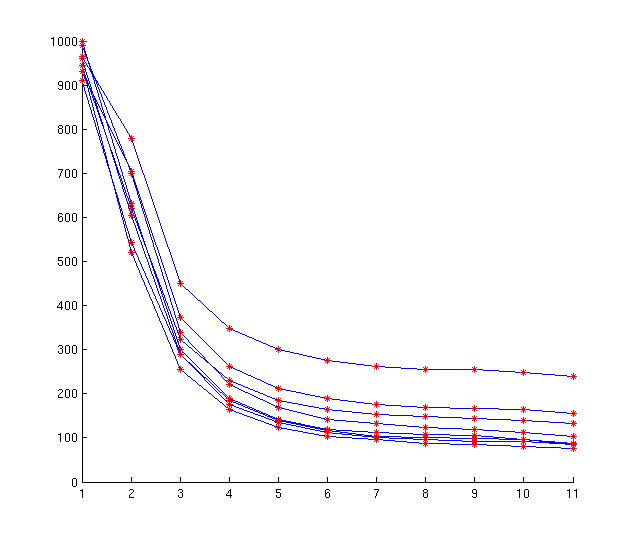
\includegraphics[width=\textwidth]{irvals}
  \end{minipage}
  \hspace{0.5cm}
  \begin{minipage}[b]{0.45\linewidth}
    \centering
    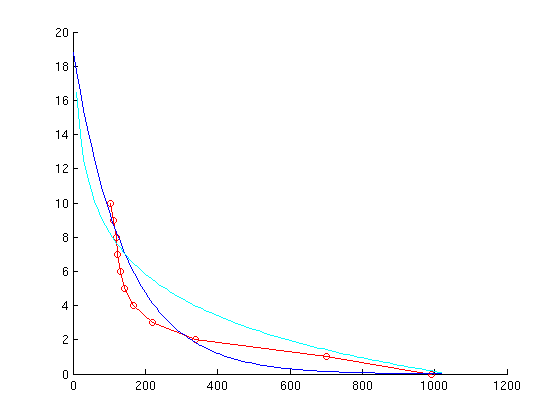
\includegraphics[width=\textwidth]{fitgraph}
  \end{minipage}
  \label{irvalsfitgraph}
  \caption{Left: Sensor values over distance, from 1 to 10 cm. The curve ``flattens'' at values larger than 7cm. Right: Red graph shows sensor values for one of the IR sensors on the Khepera, blue graph is the exponential fit, cyan is the logarithmic fit. (Source: WolframAlpha.com)}
\end{figure}

The movement of particles is governed by a random variable in the normal distribution with a a relatively small standard deviation relative to the robot movements since last loop iteration. This is a deviation from D. Oliveiras work which used a constant standard deviation relatively large to it's movement space. The particles are resampled once every 10th control loop iteration, making it on average once every 4.82 seconds (\(10* 0.482\text{ seconds}\)) and given our experience with odometry, on a run of this length of time, odometry is generally fairly accurate allowing us to use a smaller standard deviation and the smaller the movement the higher the accuracy and the lower the standard deviation. Each particle is also checked for nearby collisions making sure it doesn't move inside obstacles our outside walls. While this is not strictly necessary it emulates the real behaviour of the robot better.

\begin{figure}[ht!]
  \begin{minipage}[b]{0.45\linewidth}
    \centering
    \setlength\fboxsep{0pt}
    \setlength\fboxrule{1pt}
    \fbox{\includegraphics[width=0.95\textwidth]{pf1}}
  \end{minipage}
  \hspace{0.5cm}
  \begin{minipage}[b]{0.45\linewidth}
    \centering
    \setlength\fboxsep{0pt}
    \setlength\fboxrule{1pt}
    \fbox{\includegraphics[width=0.95\textwidth]{pf2}}
  \end{minipage}
\end{figure}
\begin{figure}[ht!]
  \begin{minipage}[b]{0.45\linewidth}
    \setlength\fboxsep{0pt}
    \setlength\fboxrule{1pt}
    \fbox{\includegraphics[width=0.95\textwidth]{pf3}}
  \end{minipage}
  \label{pfpics}
  \caption{Pictures from left to right, top to bottom, show the particle filter over a 1 minute sequence at 30 seconds interval (0, 30 and 60 seconds). In this example there were no mis-detections.}
\end{figure}

\subsection{Potential Field}
To navigate through the arena, we had to find a method which would work with our continuous map, which meant that certain methods like A* path search were out of the question. The potential field method we use was a close solution since we already had a movement method from the last task which takes an angle relative to the robot and translates it into relative wheel speeds (Motor Schema Architecture, Arkin 1989). Again, due to the fact that our map is not discretised, we found it easier to not precompute the potential field, but instead calculate the vector, which gives the direction the robot should move in, in real-time.

Our potential field method uses attracting forces from our target sources and repulsing forces from obstacles to calculate a vector which represents the direction the robot should move into. To easily calculate the repulsing forces from object, we place points along their boundary walls with a 1cm spacing (Figure \ref{potfieldmap}) and then calculate the difference vector between them and the robot position, while increasing the influence of the obstacles exponentially, the closer the robot gets to them. The attracting force of the target on the other hand --- the target being either a target point for exploration, the home position, or a known food source --- is scaled linearly across the map, so that the robot always has some goal to pursue. 

\begin{figure}[!ht]
 \centering
  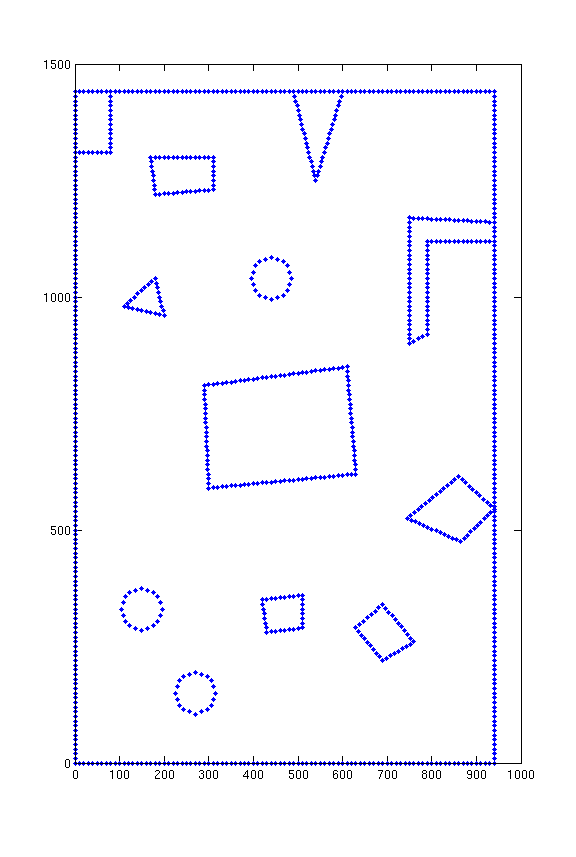
\includegraphics[width=0.7\textwidth]{potfieldmap}
  \caption{Map over the arena with the density of potential field vectors as points.}
\label{potfieldmap}
\end{figure}

In the last task, we had already developed a method to translate an angle relative to the robot into relative wheel speeds, although for the last task this angle was computed from the weighted average of the ambient light sensors. Given the angle from the our potential field, we simply inhibit one of the wheels according to the direction and size of the angle.

Overall, this method is quite simple, relatively quick, since it only needs to check a few points, and relies only on a few variables --- the distribution of the repelling points, their repelling force as well as the attracting force of the target --- so configuration was finished within a few test runs.

\subsection{Control}
The robot is controlled by a simple hybrid architecture with two deliberative, high level, components, "explore" and "collect food", and two reactive, low level, components, "navigate/go to target" and "avoid obstacle". The high level components are chosen based on the simple condition of whether the robot knows where there is food and whether it has food in its "possession". Both conditions can change to either state throughout the robot lifetime by "forgetting" a food location, done via time-out at predicted food location, and dropping of a food item at the home location. Navigation will take care of executing the plan by performing the wheel operations based on the response from the potential field and a baseline obstacle avoidance, adapted from our previous task in this course (Task 1 - Robot avoids obstacles and follows walls.), which will reactively force movement away from an obstacle if travelled to close to it. (Figure \ref{architecture})

\begin{figure}[!ht]
 \centering
  \includegraphics[width=0.5\textwidth]{architecture}
  \caption{Hybrid robot control architecture}
\label{architecture}
\end{figure}


\subsubsection{Target planning}
When the robot starts from its initial position, the control code will first set a random position as the target so that the robot starts exploring. If the robot is unable to reach the target within 15 seconds, a new random position within the arena is chosen. If the robot encounters a food source during exploration --- as specified by blocking all of its IR-sensors --- it will store that position and return home. Once it has reached home it will return to the last food position and repeat the process unless it finds a new food position on it's path. If it thinks it's reached the food position but the collection event is not triggered, in 5 seconds intervals it will place a new target at a random position within 4 cm radius around the food source to explore around that position. If after 35 seconds since it first arrived at the food source the collection event is still not triggered the food source will be removed from the robots memory and the robot will either move to another known food position or resume exploration of the map.

\subsection{Experimental methods}
To record and evaluate the performance of our robot in the given task we performed 10 subsequent runs of 3 minutes each in the actual arena to be used during the demonstration. The robot was however artificially constricted to the lower half of the arena to mitigate for the shorter runs. There were 5 food source locations reachable by the robot. The home position was a circle of approximately 11 cm radius and the robot was considered home if it stopped and flashed its LED lights when fully inside the circle. Food sources were spots on the arena of approximately 5mm radius and the food collection event was performed when any part of the robot passed on top of them. "Points" were calculated by giving 1 point for each food source reached/found and 5 points for each food item returned home.

\section{Results}
\begin{table}
 \begin{tabular}{| r | c | r | r | r |}
  \hline
  \# & Time to 1st food & Points & Mis-predictions & \# of resamplings \\
  \hline
  1 & -- & 0 & 4 & 44 \\ 
  2 & 1:06 min & 13 & 1 & 38 \\
  3 & 2:10 min & 7 & 0 & 35 \\
  4 & -- & 0 & 7 & 42 \\
  5 & 45 sec & 13 & 1 & 41 \\
  6 & -- & 0 & 8 & 35 \\
  7 & -- & 0 & 5 & 37 \\ 
  8 & -- & 0 & 0 & 46 \\
  9 & -- & 0 & 2 & 42 \\
  10 & 20 sec & 7 & 0 & 37 \\
  \hline \hline
  Sum: & ~ & 40 & 28 & 397 \\
  \hline
 \end{tabular}
 \label{exptable}
 \caption{Results over 10 runs of 3 minutes each.}
\end{table}


Once a food source was found, our robot performed well, with an average of 10 points over those runs. However, only 40\% of the runs actually found any food source at all lowering the point average to 4 points per run.

The particle filter showed very good results however throughout all tests, giving an average 93\% correct prediction. The longest sequence of incorrect resamplings in our test set was 5 resamplings before it found the correct location again. This amounts to approximately 30 consecutive seconds at which the robot was incorrectly localised (\(1.87s * 5 + (0.482s * 10 * 5) = 30.035s\)). One other case had 3 consecutive mis-predictions but most other incorrect localisations were corrected in the next resampling step.

On average each timestep (control loop iteration) took 0.546s, with an average resampling time of 1.187s once every 10 timesteps and 0.482s for the rest of the loop. The resampling time was largely dominated by the calculation of predicted IR values using line intersection. This process took 4.9ms per particle, adding up up to 980ms for 200 particles, i.e. ~82.6\% of the whole timestep. The times were calculated by timing each component of each run and averaging over all the runs.

\section{Discussion}
We can show that by solving the individual problems of navigation, localisation and control we can make a Khepera robot perform a task involving multiple goals in a predefined arena. The robot performs as expected, can localise itself reliably and can complete the task specified but falls short on one main aspect, the discovery of food sources. This stems from two underlying problems: the speed of the robot and the exploratory behaviour.

The average time for each control loop when it's not resampling is almost half a second, forcing us to use a slower movement speed for our robot simply due to the low update frequency. As we can only send commands to the robot once each timestep, at a higher speed, the robot would move further before a new command is transmitted and thus lose precision. Additionally, every 10 iterations a pause of an average 1.187 seconds would occur due to the particle filter resampling at which the robot doesn't move at all, further slowing down its behaviour.

\subsection{Map and exploration/control}
To help the robot find food quicker, a heuristic approach could've been used for exploration instead of the simple, naive, stochastic approach. For example, as a simple extension the map could've been divided in sections of equal area of empty space (space not covered by an obstacle) approximating the surface area of the robot base (for example, 2 * robot diameter). This information can be precomputed and stored as a separate map. Now, in robot exploration mode instead of choosing an arbitrary random location it will pick the closest location from the list of map sections and make sure to pick a new one each time until all have been visited. This would allow a more reliable coverage of the arena with a higher expectation of finding a food source.

\subsection{Localisation}
In terms of accuracy the particle filter performs as desired, but when it comes to speed of calculation there is much that could be improved.

By far the slowest operation in our particle filtering (and our control in general) is the calculation simulated IR-values for each of the particles. This was greatly reduced by reducing the number of walls the prediction of the IR-values for each particle would take into account as well as only resampling every ten loop iterations. Still, the operation is one of mathematical nature that can most certainly be improved directly, by, for example, making better use of matlabs powerful matrix operations.

Mathematics aside the speed performance can also be indirectly improved by using a dynamic number of particles. The number could start relatively low (100 for example) and increase or decrease, with a hard floor and ceiling, depending on the certainty of each prediction. This would need to be balanced properly as too few particles can drastically reduce prediction performance and intermittently lose valuable information.

We did, however, find that resampling only every so often has an added benefit for our system. Since the information the IR-sensors provide is limited, resampling too often at positions where there is no input from them would add too much noise to the particles, reducing prediction accuracy.
\subsection{Navigation}
While the potential field worked for our simple purposes of navigation it too can be improved to increase robot efficiency. It did make the robot reliably avoid obstacles and move between them, but once a larger obstacle directly blocked the path to the target, given that we calculate the vectors in a simple, linear way, repulsing directly away from obstacles and attracting directly towards the goals, this would point the robot straight towards an obstacle if a target was directly behind it.

For all intents and purposes, the functionality it provided was reasonable and its simplicity meant that we did not have to spend much time on tweaking it.
\subsection{Finally}
To conclude, this exercise has illustrated how well methods like particle filtering can work, even with minor sensory information, in predicting an accurate robot pose in a pre defined arena. We can also take away that, while functional soundness is important, so is efficiency and method of implementation. Something like a slower algorithm can propagate through the entire implementation and force a change of strategy that could have otherwise been avoided.

\begin{thebibliography}{9}
\bibitem{oliveira}
  Danilo Oliveira,
  \emph{Particle Filter Implementation in Matlab},
  ai-class.com,
  2011,
  \url{http://www.youtube.com/watch?v=sjny6-lVtb4}.
\bibitem{aiclass}
  Peter Norvig, Sebastian Thrun,
  2012,
  \emph{Introduction to Artificial Intelligence},
  Udacity, Stanford Engineering,
  \url{http://www.ai-class.com}.
\end{thebibliography}
\section{Appendix}
\subsection{Code listing}
\subsubsection{Run.m}
\lstinputlisting{Run.m}
\subsubsection{initialize.m}
\lstinputlisting{initialize.m}
\subsubsection{control.m}
\lstinputlisting{control.m}
\subsubsection{ressample.m}
\lstinputlisting{ressample.m}
\subsubsection{weights.m}
\lstinputlisting{weights.m}
\subsubsection{probdensity.m}
\lstinputlisting{probdensity.m}
\subsubsection{moveParticles.m}
\lstinputlisting{moveParticles.m}
\subsubsection{predictIRNew.m}
\lstinputlisting{predictIRNew.m}
\subsubsection{distance.m}
\lstinputlisting{distance.m}
\subsubsection{getPotFieldMap.m}
\lstinputlisting{getPotFieldMap.m}
\subsubsection{getPotFieldVec.m}
\lstinputlisting{getPotFieldVec.m}
\subsubsection{odometry.m}
\lstinputlisting{odometry.m}



%%% End document
\end{document}
